To uncover the elusive extent repair bug in Azure Storage vNext, its developers wrote a testing harness in \psharp. The developers of vNext expected that it was more likely for the bug to occur in the ExtMgr logic, rather than the EN logic. Hence, the testing harness focuses on the real ExtMgr using mocked ENs.

The testing harness consists of the following \psharp machines (as shown in Figure~\ref{fig:azurestoremodel}):
%\begin{enumerate}
\begin{description}
\item[ExtentManager] acts as a thin wrapper machine for the real ExtMgr component in vNext.

\item[ExtentNode] represents a simplified mocked EN.

\item[TestingDriver] communicates with all other machines, relays messages between the \texttt{ExtentManager} and the \texttt{ExtentNode} machines, and is responsible for driving testing scenarios.

\item[RepairMonitor] collects states from all \texttt{ExtentNode} machines in the testing harness and checks desired properties, such as that an extent is replicated or repaired at the expected ENs.
\end{description}

\begin{figure}[t]
\centering
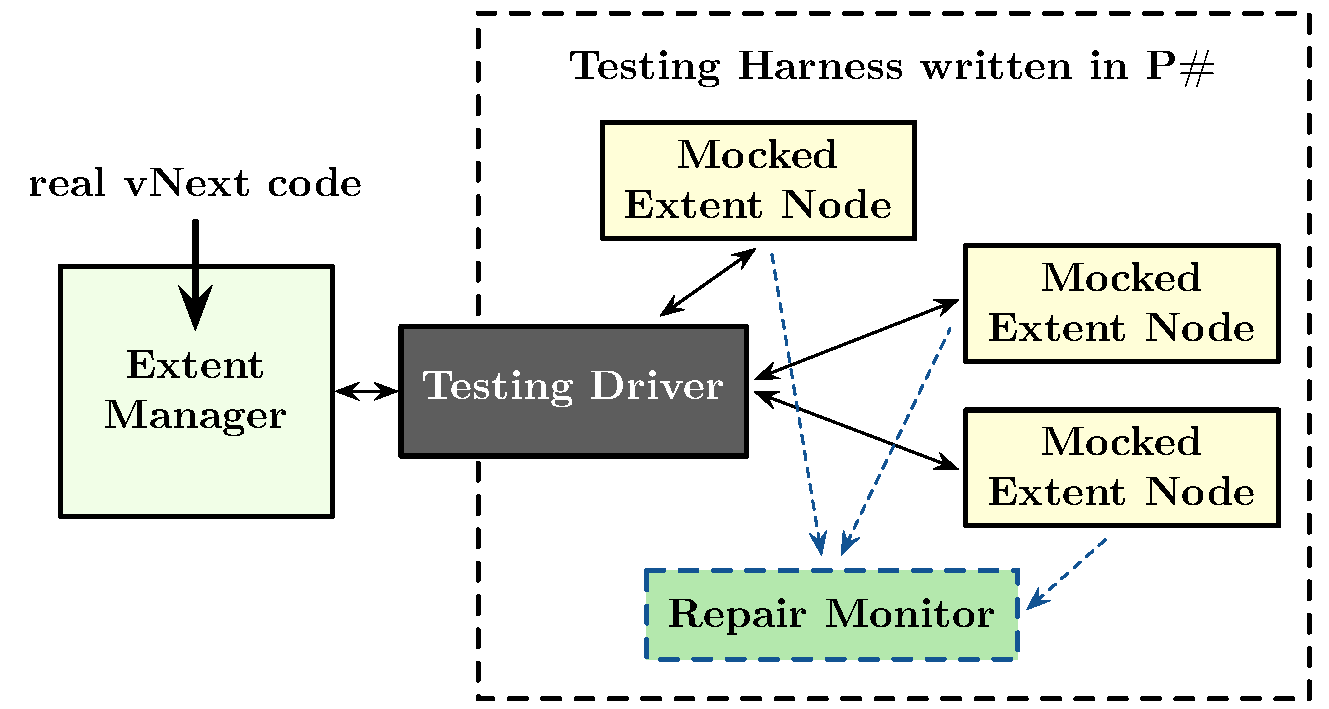
\includegraphics[width=\linewidth]{img/mocked_vnext}
\caption{Real Extent Manager with a mocked environment (each box represents one \psharp machine).}
\label{fig:azurestoremodel}
\end{figure}

\subsection{The ExtentManager machine}
\label{sec:method:wrap_target}

The real ExtMgr in vNext, which is our system-under-test, is wrapped inside the \texttt{ExtentManager} \psharp machine in the testing harness.

\begin{figure*}[t]
\centering
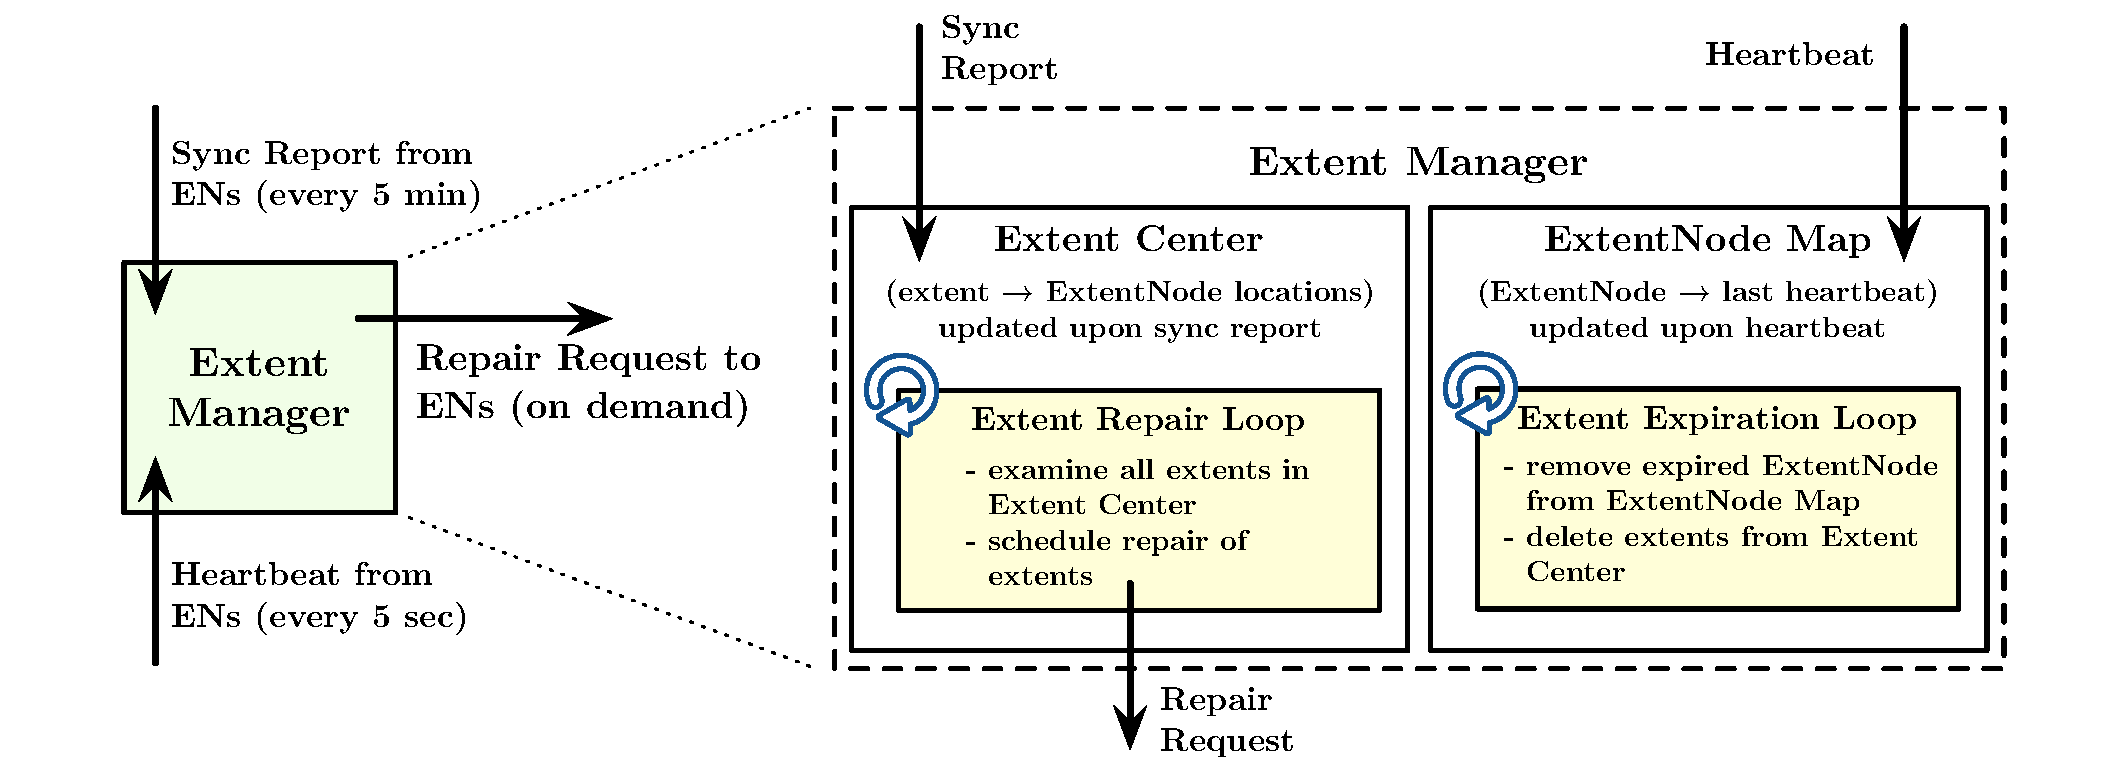
\includegraphics[width=.9\linewidth]{img/extent_manager}
\caption{Internal components of the real Extent Manager in Azure Storage vNext.}
\label{fig:extentmanager}
\end{figure*}

\textbf{Internals of the real Extent Manager}.
Inside the real ExtMgr (see Figure~\ref{fig:extentmanager}), there are two data structures related to extent replication and repair: \texttt{ExtentCenter} and \texttt{ExtentNodeMap}. The \texttt{ExtentCenter} maintains the mapping records from extents to their hosting ENs. It is updated upon the periodic sync reports from the ENs. Recall that the sync report from a particular EN lists all the extents stored at the EN. Its purpose is to update extent manager's possible out-of-date view of the EN with the ground truth. The EN map records the latest heartbeat time from every EN.

The ExtMgr runs internally a periodic {\em EN expiration loop} that is responsible for removing ENs that have been missing heartbeats for an extended period, as well as cleaning up the corresponding records in the \texttt{ExtentCenter}. In addition, the ExtMgr runs a periodic {\em extent repair loop} that examines all the \texttt{ExtentCenter} records, identifies extents with missing replicas, schedules extent repair tasks and sends them to the ENs.

\textbf{Intercepting messages between machines}.
The real ExtMgr uses a network engine to send messages to the ENs. The testing harness mocks the original network engine in vNext and overrides its interface. In this way, the mocked network engine intercepts all outbound messages and relays them to the \texttt{TestingDriver} machine, which is responsible for dispatching the messages to the corresponding \texttt{ExtentNode} machines. As shown in Figure~\ref{fig:enginecode}, the mocked network engine intercepts the outbound messages from the ExtMgr and invokes \texttt{PSharpRuntime.Send(...)} to asynchronously relay the messages to \texttt{TestingDriver}. Conceivably, the mocked network engine could leverage the nondeterminism support in \psharp and choose to drop the messages in a non-deterministic fashion, in case emulating message loss is desirable.

%Method dispatch is the process of selecting which method, from a set of available methods with the same interface, should be invoked during a program's execution. There are two types of method dispatch: \emph{static}, which is resolved during compilation; and \emph{dynamic}, which is resolved in runtime.  \csharp (and thus \psharp) supports both static and dynamic dispatch, and provide the \texttt{virtual} modifier that can be used to declare a method which can be \emph{overridden} during runtime by an inheriting class. This capability is provided by the common language runtime (CLR) of Microsoft's .NET framework, and is a key feature of \csharp as well as other mainstream object-oriented languages.

%Using method dispatch for modeling is straightforward. The system-under-test exposes a set of APIs as \emph{virtual methods}. The developer can then \emph{override} these APIs and replace them with \emph{mocks} that will execute instead of the original implementations during systematic testing with \psharp.

%\begin{figure}[t]
%\begin{lstlisting}
%// Public interface of the real network engine
%class NetworkEngine {
  %public virtual void SendMessage(Socket s, Message msg);
  %public virtual void EnqueueMessage(Message msg);
%}
%
%// The mocked network engine used during testing
%class MockedNetEngine : NetworkEngine {
  %ExtentManager EM; // Handle to actual system-under-test
  %MachineId Env; // Handle to modeled environment
  %
  %public MockedNetEngine(ExtentManager em, MachineId env) {
    %this.EM = em;
    %this.Env = env;
  %}
  %
  %public override void SendMessage(Socket s, Message msg) {
    %PSharpRuntime.Send(this.Env, new MsgEvent(), s, msg);
  %}
  %
  %public override void EnqueueMessage(Message msg) {
    %this.EM.ProcessMessage(msg);
  %}
%}
%\end{lstlisting}
%\vspace{-2mm}
%\caption{The mocked network engine used for testing the Azure Storage vNext system.}
%\label{fig:enginecode}
%%\vspace{-2mm}
%\end{figure}

\begin{figure}[t]
\begin{lstlisting}
// network interface in vNext
class NetworkEngine {
  public virtual void SendMessage(Socket s, Message msg);
}

// mocked engine for intercepting Extent Manager messages
class MockedNetEngine : NetworkEngine {
  public override void SendMessage(Socket s, Message msg) {
    // intercept and relay Extent Manager messages
    PSharpRuntime.Send(this.TestingDriver,
      new MessageFromExtentManagerEvent(), s, msg);
  }
}
\end{lstlisting}
\vspace{-2mm}
\caption{Mocked network engine in vNext.}
\label{fig:enginecode}
%\vspace{-2mm}
\end{figure}

%We now give an example of using dynamic dispatch to model the network engine of an extent manager in the Azure Storage vNext case study (see Figure~\ref{fig:enginecode}). The network engine is responsible for sending to and receiving messages from the various components of the system. During real execution, the network engine uses a custom remote procedure call (RPC) .NET library for communication. For testing, though, it is desirable to replace all calls to this RPC library with \psharp send and receive operations, which can be captured and systematically interleaved to find bugs. We easily achieved this by exposing the original send message operation of the network engine as a virtual method, and then overriding it for testing. In the overridden method, we created a \psharp event and then we wrapped the original message in this event's payload. Then, instead of invoking the RPC library, we invoke the \texttt{PSharpRuntime.Send(...)} method, which asynchronously sends the event (containing the original message) to the target extent node machine.

%For mocking the receive operation, we take advantage of the implicit receive of events in \psharp machines. When a extent node machine receives an event, an appropriate event handler is invoked, which extracts the original message from the payload and then handles it accordingly.

\textbf{Specifics of the ExtentManager machine}.
Figure~\ref{fig:wrap_target} shows code snippets from the \texttt{ExtentManager} \psharp machine. \texttt{ExtentManager} is a thin wrapper of the real ExtMgr. The mocked network engine replaces the real one in ExtMgr, intercepts all the outbound messages from ExtMgr and relays them to \texttt{TestingDriver}.

%A typical wrapper machine contains a handle (as a field) to the system component that is being wrapped (in our case the real Extent Manager object) and the event handlers are responsible for translating any received events to method calls in the real code that is being tested. The \texttt{ExtentManager} is accompanied by a mocked version of the real Network Engine class. The real Extent Manager is communicating with the outside world via remote procedure calls, but in \psharp harness we want to capture this communicating and expose it as calls to \psharp communicating primitives. This is discussed in detail in \S\ref{sec:method:model:dispath}.

%As shown in Figure~\ref{fig:wrap_target}, the \texttt{ExtentManagerMachine} is a wrapper machine and is used to connect the \psharp modeled code with the legacy \csharp code. A typical wrapper machine contains a handle (as a field) to the system component that is being wrapped (in our case the real Extent Manager object) and the event handlers are responsible for translating any received events to method calls in the real code that is being tested. The \texttt{ExtentManager} is accompanied by a mocked version of the real Network Engine class. The real Extent Manager is communicating with the outside world via remote procedure calls, but in \psharp harness we want to capture this communicating and expose it as calls to \psharp communicating primitives. This is discussed in detail in \S\ref{sec:method:model:dispath}.

\begin{figure}[t]
\begin{lstlisting}
// Wrapping the target vNext component in a P# machine
class ExtentManagerMachine : Machine {
  private ExtentManager extMgr; // real vNext code

  void Init() {
    extMgr = new ExtentManager();
    extMgr.netEngine = new MockedNetEngine(); // mock network
    extMgr.isMockingTimer = true;	 // disable internal timer
  }

  [OnEvent(MessageFromExtentNode, DeliverExtentNodeMessage)]
  void DeliverExtentNodeMessage() {
    var msg = (ExtentNodeMessage)this.Payload;
    // relay messages from Extent Node to Extent Manager
    extMgr.ProcessMessage(msg);
  }
	
  [OnEvent(TimerTick), nameof(ProcessExtentRepair))]
  void ProcessExtentRepair() {
    // extent repair loop driven by external timer
    extMgr.ProcessEvent(new ExtentRepairEvent());
  }
}
\end{lstlisting}
\vspace{-2mm}
\caption{System-under-test: instance of the real Extent Manager wrapped inside the \texttt{ExtentManager} machine.}
\label{fig:wrap_target}
%\vspace{-2mm}
\end{figure}

Messages coming from the ENs do \emph{not} go through the mocked network engine. They are delivered to the \texttt{ExtentManager} machine directly and trigger an action that invokes the messages on the internal ExtMgr with \texttt{extMgr.ProcessSingleMessage}. The benefit of this approach is that ExtMgr can be tested without modifying its code; ExtMgr is simply unaware of the testing harness and behaves as if it running in a real distributed environment and communicating with real ENs.

System correctness should \emph{not} hinge on the frequency of any individual timer. Instead, all nondeterminism due to timing-related events must be delegated to \psharp. To achieve this, all timers inside ExtMgr are disabled, and the EN expiration loop and the extent repair loop are driven instead by timers modeled in \psharp, an approach that was used in previous work~\cite{desai2015building}. The \psharp timers send nondeterministic timeout events that are controlled by the \psharp runtime. Hence, the \psharp testing engine has the freedom to schedule arbitrary interleavings between timeout events and all other regular system events.

\subsection{The ExtentNode machine}
\label{sec:method:mock_en}

The \texttt{ExtentNode} machine is a simplified version of the original EN. The machine omits much of the complex details of a real EN, and only mocks the logic necessary for the testing scenarios. This mocked logic includes: repairing an extent from its replica, and sending sync reports and heartbeat messages periodically to the \texttt{ExtentManager} machine.

The testing harness leverages components of Azure Storage vNext whenever it is appropriate. For example, the \texttt{ExtentNode} machine re-uses the \texttt{ExtentCenter} data structure, a component that is used inside a real EN for extent bookkeeping.

In the mocked extent repair logic, \texttt{ExtentNode} takes action upon receiving an extent repair request from the \texttt{ExtentManager} machine. It sends a copy request to a source \texttt{ExtentNode} machine where a replica is stored. After receiving an \texttt{ExtentCopyResponse} event from the source, it updates the internal \texttt{ExtentCenter}, as illustrated in Figure~\ref{fig:mocked_en}. 

In the mocked EN sync logic, the machine is again driven by an external timer provided by \psharp. It prepares a sync report with \texttt{extCtr.GetSyncReport(...)} and asynchronously sends the report to \texttt{ExtentManager} with \texttt{PSharpRuntime.Send(...)}.

%\begin{figure}[t]
%\begin{lstlisting}
%// Wrapping the target vNext component in P#
%class ExtentNodeMachine : Machine {
  %private ExtentNode.ExtentCenter extCtr; // real vNext component
%
	%[OnEventDoAction(typeof(RepairExtentRequestEvent), nameof(ProcessRepairExtentRequest))]
	%[OnEventDoAction(typeof(DownloadExtentRequestEvent), nameof(ProcessDownloadExtentRequestEvent))]
	%[OnEventDoAction(typeof(DownloadExtentResponseEvent), nameof(ProcessDownloadExtentResponseEvent))]
	%[OnEventDoAction(typeof(TimerTickEvent), nameof(ProcessExtentNodeSyncEvent))]
%
  %void ProcessRepairExtentRequest()
  %{
    %var source = GetRepairSourceMachine(this.Payload);
    %PSharpRuntime.Send(source, new DownloadExtentRequestEvent(), this.Payload);
  %}
%
  %void ProcessDownloadExtentRequestEvent()
  %{
	  %var destination = GetRepairDestinationMachine(this.Payload);
    %var ext_id = GetExtentID(this.Payload);
    %
		%Extent ext;
    %if (extCtr.TryGet(ext_id, out ext))
      %PSharpRuntime.Send(destination, new DownloadExtentResponseEvent(), ext);
  %}
%
  %void ProcessDownloadExtentResponseEvent()
  %{
    %var ext = (Extent)this.Payload;
    %extCtr.AddExtent(ext);
%
    %this.Monitor<RepairMonitor>(new NotifyExtentRepairCompletion(), this.NodeID);
  %}
%
  %void ProcessExtentNodeSyncEvent()
  %{
    %var sync = new ExtentNodeSync(this.NodeID);
    %extCtr.Extents.ForEach(ext =>
      %{
        %var rec = new ExtentRecord(ext.ExtentID, ext.Length, ext.Sealed);
        %sync.ExtentRecs.Add(rec);
      %});
    %PSharpRuntime.Send(this.NameNode, new NameNodeMessageEvent(), sync);
  %}
%}
%\end{lstlisting}
%\vspace{-2mm}
%\caption{Mocked Extent Node.}
%\label{fig:mocked_en}
%%\vspace{-2mm}
%\end{figure}

%\begin{figure}[t]
%\begin{lstlisting}
%// Mocking Extent Node in P#
%class ExtentNodeMachine : Machine {
  %// use real vNext component whenever appropriate
  %private ExtentNode.ExtentCenter extCtr;
%
  %[OnEventDoAction(typeof(RepairExtentRequestEvent), nameof(ProcessRepairExtentRequest))]
  %[OnEventDoAction(typeof(TimerTickEvent), nameof(ProcessExtentNodeSync))]
%
  %// extent repair logic
  %void ProcessRepairExtentRequest()
  %{
    %var source = GetRepairSourceMachine(this.Payload);
    %PSharpRuntime.Send(source, new DownloadExtentRequestEvent(), this.Payload);
  %}
  %...
%
  %// extent node sync logic
  %void ProcessExtentNodeSync()
  %{
    %var sync = new ExtentNodeSync(this.NodeID);
    %extCtr.Extents.ForEach(ext =>
      %{
        %sync.ExtentRecords.Add(new ExtentRecord(ext));
      %});
    %PSharpRuntime.Send(this.ExtentManagerMachine, new MessageFromExtentNodeEvent(), sync);
  %}
%}
%\end{lstlisting}
%\vspace{-2mm}
%\caption{Mocked Extent Node.}
%\label{fig:mocked_en}
%%\vspace{-2mm}
%\end{figure}

\begin{figure}[t]
\begin{lstlisting}
// Mocking Extent Node in P#
class ExtentNodeMachine : Machine {
  // leverage real vNext component whenever appropriate
  private ExtentNode.ExtentCenter extCtr;

  // extent repair logic
  ...
  [OnEvent(ExtentCopyResponse, ProcessExtentCopyResponse)]
  void ProcessExtentCopyResponse() {
    // extent copy response from source replica
    if (IsCopySucceeded(this.Payload)) {
      var rec = GetExtentRecord(this.Payload);
      extCtr.AddOrUpdate(rec); // update Extent Center
    }
  }

  // extent node sync logic
  [OnEvent(TimerTick, ProcessExtentNodeSync)]
  void ProcessExtentNodeSync() {
    var sync = extCtr.GetSyncReport(); // prepare sync report
    PSharpRuntime.Send(this.ExtentManagerMachine,
      new MessageFromExtentNodeEvent(), sync);
  }
}
\end{lstlisting}
\vspace{-2mm}
\caption{The mocked EN in vNext.}
\label{fig:mocked_en}
%\vspace{-2mm}
\end{figure}

\subsection{The TestingDriver machine}
\label{sec:method:driver}

The \texttt{TestingDriver} machine drives two testing scenarios. In the first scenario, it launches one \texttt{ExtentManager} and three \texttt{ExtentNode} machines, with a single extent on one of the ENs. It waits for the extent to be replicated at the other ENs. In the second scenario, it fails one of the \texttt{ExtentNode} machines and launches a new one. It waits for the extent to be repaired on the new EN. We omit illustrative code snippets due to space constraints.

\subsection{The RepairMonitor machine}
\label{sec:method:monitor}

The \texttt{RepairMonitor} machine is a \psharp liveness monitor (see \S\ref{sec:bg:bugs}) that transitions between a cold and a hot state. Whenever an extent node fails, \texttt{RepairMonitor} is notified. As soon as the number of extent replicas falls below a specified target (three replicas in the current test harness), \texttt{RepairMonitor} transitions into the hot \emph{repairing} state, where the missing replica is being repaired. Whenever a replica is repaired, the \texttt{RepairMonitor} machine is also notified. It transitions into the cold \emph{repaired} state, when the replica number reaches again the target, as illustrated in Figure~\ref{fig:monitor}.

In the extent repair testing scenarios, \texttt{RepairMonitor} checks that it should {\em always eventually} end up in the cold repaired state. Otherwise, the \texttt{RepairMonitor} machine is stuck in the hot repairing state for {\em infinitely} long. This indicates that the corresponding execution sequence results in an extent replica never being repaired, which is a liveness bug.

\begin{figure}[t]
\begin{lstlisting}
class RepairMonitor : Monitor {
  // true: EN has replica, false: EN has no replica
  private Dictionary<Machine, bool> ExtentNode2Replica;

  // cold state: repaired
  [OnEvent(NotifyEnFailure, ProcessExtentNodeFailure)]
  cold state Repaired {
    void ProcessExtentNodeFailure() {
        var node = GetExtentNode(this.Payload);
        ExtentNode2Replica.Remove(node);
        goto Repairing;
    }
  }

  // hot state: repairing
  [OnEvent(NotifyExtentRepaired, ProcessExtentRepaired)]
  hot state Repairing {
    void ProcessExtentRepaired() {
      var node = GetExtentNode(this.Payload);
      ExtentNode2Replica[node] = true;
      if (ReplicaCount == Harness.REPLICA_COUNT_TARGET)
        goto Repaired;
    }
  }
}
\end{lstlisting}
\vspace{-2mm}
\caption{The RepairMonitor machine.}
\label{fig:monitor}
%\vspace{-2mm}
\end{figure}

\subsection{Liveness Bug in Azure Storage vNext}
\label{sec:method:azurestore}

It took less than ten seconds for the \psharp testing engine to report the first occurrence of a liveness bug in vNext (see \S\ref{sec:eval}). Upon examining the debug trace, the developers of vNext were able to quickly confirm the bug.

However, the original \psharp trace did not include sufficient detail to allow the developers to identify the root cause of the problem. Fortunately, running the test harness took very little time, so the developers were able to quickly iterate and add more refined debug outputs in each iteration. After several iterations, the developers were able to pinpoint the exact culprit and immediately propose a solution for fixing the bug. Once the proposed solution was implemented, the developers ran again the test harness. No bugs were found during 100,000 iterations, a process that required only tens of minutes.

The liveness bug occurs in the second testing scenario, where the \texttt{TestingDriver} fails one of the \texttt{ExtentNode} and launches a new one. The \texttt{RepairMonitor} transitions to the hot repairing state and is stuck in the state for infinitely long.

The following is one particular execution sequence resulting in this liveness bug: (i) EN$_0$ fails and is detected by the EN expiration loop; (ii) EN$_0$ is removed from the EN map; (iii) the extent center is updated and the replica count drops from 3 (which is the target) to 2; (iv) ExtMgr receives a sync report from EN$_0$; (v) the extent center is updated and the replica count increases again from 2 to 3. This is problematic since the replica count is equal to the target, which means that the extent repair loop will never schedule any repair task. At the same time, there are only two \emph{true} replicas in the system, which is one less than the target. This execution sequence leads to one missing replica; repeating this process two more times would result in all replicas missing, but ExtMgr still thinking that all replicas are healthy. In production, such a bug can cause a very serious incident of customer data loss.

The culprit is in (iv), where ExtMgr receives a sync report from EN$_0$ after deleting the EN. This may occur in \psharp due to arbitrary interleaving of events. It may also occur, albeit much less frequently, during stress testing due to messages being delayed in the network. This explains why the bug only occurs from time to time during stress testing and requires long executions to manifest. In contrast, \psharp allows the bug to manifest quickly, the developers to iterate rapidly, the culprit to be identified promptly, and the fix to be tested effectively and thoroughly, all of which have the potential to vastly increase the productivity of distributed storage system development.

%%\subsection{Modeling the environment}
%\subsection{Test Harness}
%\label{sec:method:model}
%
%The environment of a distributed system might consist of other distributed systems and services, clients, operating system timers, as well as libraries for networking or other purposes. To be able to systematically test a distributed system, this environment must be modeled and all the interactions between the environment and the system, as well as all the nondeterminism, must be captured and controlled by the \psharp runtime.
%
%%\subsubsection{Creating a test harness using \psharp}
%\subsubsection{Orchestrating Machines}
%\label{sec:method:model:harness}
%
%\begin{figure}[t]
%\centering
%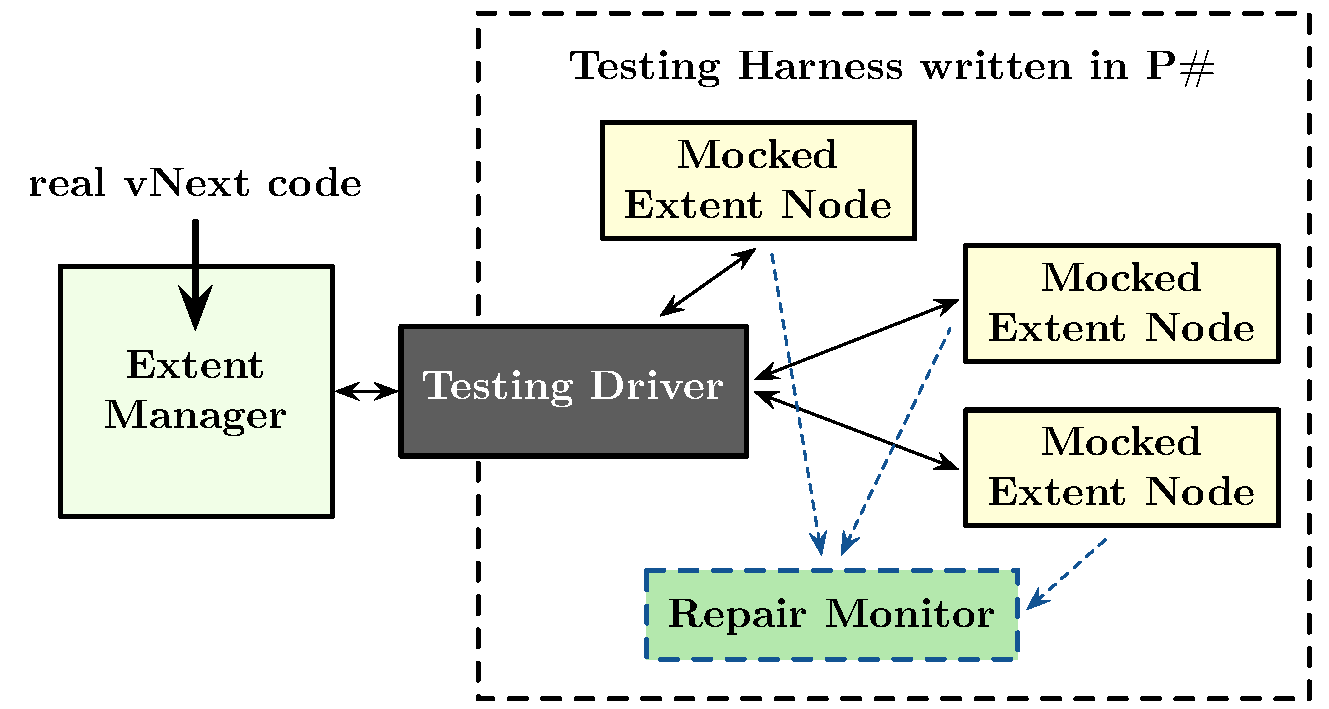
\includegraphics[width=\linewidth]{img/mocked_vnext}
%\caption{The real environment of the Extent Manager is replaced with a mocked version for testing.}
%\label{fig:azurestoremodel}
%\end{figure}
%
%Before being able to use \psharp to test an existing distributed system, the environment of the components that the developer wants to test have to be modeled using the \psharp state machine APIs.  This involves creating mock classes that inherit from the \texttt{Machine} abstract class. The \texttt{Machine} class exposes methods for declaring a state machine (e.g. machine states and state transitions) as well as methods for sending events to other machines, declaring event handlers for received events, and accessing the payload from the latest received event.
%
%In the Azure Storage vNext case study, we created the following \psharp machines: \texttt{Environment}, \texttt{ExtentNode}, \texttt{ExtentManager}, and \texttt{Timer}.
%
%The \texttt{Environment} (denoted with a dashed line box in Figure~\ref{fig:azurestoremodel}) is essentially a ``god'' machine: it is the very first machine that is created; has a handle to all other machines in the harness; and includes the logic based on which the test harness will execute. The programmer is free to create either a finite test harness (e.g. with a predefined number of node failures) or an infinite test harness (e.g. with an unbounded number of failures), as long as any nondeterminism (e.g. when to insert a failure) is captured using the available \psharp APIs.
%
%Finally, the \texttt{Timer} machine models the operating system timer and is responsible for triggering events related to the Azure Storage vNext logic (e.g. synchronization messages, heartbeats and repair logic loops). This is discussed in detail in \S\ref{sec:method:model:timers}.
%
%\subsubsection{Modeling and injecting failures}
%\label{sec:method:model:failures}
%
%In production, each Extent Node of the Azure Storage vNext system periodically (every 5 seconds) sends a heartbeat to the Extent Manager which notifies that the Extent Node is alive. Because we want to model failures and systematically inject them using \psharp, we abstract away the heartbeat mechanism in our harness. However, the Extent Manager logic relies on time intervals to detect node failures (see Figure~\ref{fig:expiration}). The way to abstract this time-related logic and connect the real code with the modeled code is to use virtual dispatch and override the virtual \texttt{IsNodeExpired} method with a mocked version.
%
%\begin{figure}[t]
%\begin{lstlisting}
%// Real code for detecting node expiration
%public virtual bool IsNodeExpired(string id, DateTime time)
%{
  %return DateTime.Compare(time, DateTime.Now) <= 0;
%}
%
%// Mocked code for detecting node expiration
%public override bool IsNodeExpired(string id, DateTime time)
%{
  %return this.DeletedNodes.Contains(id);
%}
%\end{lstlisting}
%\vspace{-2mm}
%\caption{Abstracting the node expiration logic in the Extent Manager component of Azure Storage vNext.}
%\label{fig:expiration}
%%\vspace{-2mm}
%\end{figure}
%
%Figure~\ref{fig:expiration} presents how we mocked the node expiration detection method. Instead of comparing the time interval as in the original code, we now check if the set \texttt{DeletedNodes} contains the id of the Extent Node that we are checking for expiration. If it contains the id, then it means that the node has failed. The \texttt{Environment} machine that we have created as part of our testing \psharp harness, will nondeterministically choose a node to kill, then send the id of this killed node to the Extent Manager wrapper machine, who will in turn add it to the \texttt{DeletedNodes} set.
%
%\subsubsection{Entry point to a \psharp test harness}
%\label{sec:method:model:entrypoint}
%
%A developer can specify the entry point of a \psharp test harness similar to how unit tests are typically written. Figure~\ref{fig:entrypoint} shows the source code of the entry point for the Azure Storage vNext \psharp test harness. The programmer can declare an entry point method using the \texttt{Microsoft.PSharp.Test} attribute. When the \psharp systematic testing engine is invoked, it will scan the binary and attempt to find a static method declared with this attribute. When such a method is found (in our example the \texttt{Execute()} method), the testing engine will invoke it and start testing the program. The systematic engine can optionally run multiple iterations of the test harness, each one potentially exploring a different schedule. In each iteration, the program state will be reset (any static fields must be explicitly reset by the programmer) and the entry point will be re-invoked.
%
%\begin{figure}[t]
%\begin{lstlisting}
%[Microsoft.PSharp.Test]
%public static void Execute()
%{
  %PSharpRuntime.CreateMachine(typeof(Environment));
%}
%\end{lstlisting}
%\vspace{-2mm}
%\caption{Static \csharp method acting as the entry point to the Azure Storage vNext \psharp test harness.}
%\label{fig:entrypoint}
%%\vspace{-2mm}
%\end{figure}
%
%\subsubsection{Abstracting timers}
%\label{sec:method:model:timers}
%
%Distributed systems are often using timers to determine when an event should be send from one component to another. For example, in the Azure Storage vNext system, each Extent Node is associated with a timer that fires of a synchronization message every 5 minutes and a heartbeat every 5 seconds. This timer is related to the liveness bug that we discovered: the synchronization message that gets fired every 5 minutes can potentially race with an Extent Node failure; if it arrives after the node failed, then the bug would manifest. Traditional testing techniques cannot easily find such a bug, due to the very infrequent occurrence of this race due to the timer. 
%
%Our methodology in \psharp to systematically test distributed systems that rely on timers, is to abstract timers away, model them using message passing communication and introduce nondeterminism in their firing. This nondeterminism is introduced using the \psharp \texttt{Nondet()} method, which returns a nondeterministic boolean value that is controlled by the \psharp runtime during systematic testing.
%
%Figure~\ref{fig:timer} shows how we modeled a generic timer in the Azure Storage vNext case study. The Extend Manager, as well as each Extent Node in the harness, is associated with a unique \texttt{Timer} machine. When creating this machine, we pass as a payload the id of the machine that owns this timer. When the \texttt{Timer} machine is created, it stores this id in the \texttt{Owner} field and then transitions to the \texttt{Active} state. In this state, the \texttt{Timer} loops infinitely and nondeterministically (using \texttt{Nondet()}) sends a \texttt{TimerTickEvent} to \texttt{this.Owner}. When the Extent Node owner receives this event, it handles it by generating a synchronization message that is being send to the Extent Manager. Similarly, when the Extent Manager receives a \texttt{TimerTickEvent} from its own \texttt{Timer}, it handles it by nondeterministically invoking repair-related methods in the Extent Repair Center data structure. 
%
%\begin{figure}[t]
%\begin{lstlisting}
%internal class Timer : Machine
%{
  %MachineId Owner; // Id of the owner machine
%
  %[Start]
  %[OnEntry(nameof(InitOnEntryAction))]
  %[OnEventGotoState(typeof(Unit), typeof(Active))]
  %class Init : MachineState { }
%
  %void InitOnEntryAction()
  %{
    %this.Owner = (MachineId)this.Payload;
    %// triggers state transition to Active
    %this.Raise(new Unit());
  %}
%
  %[OnEntry(nameof(ProcessTickEvent))]
  %[OnEventGotoState(typeof(Unit), typeof(Active))]
  %class Active : MachineState { }
%
  %void ProcessTickEvent()
  %{
    %// Nondeterministic boolean choice controlled by P#
    %if (this.Nondet())
      %// sends a timer tick event to the owner machine
      %this.Send(this.Owner, new TimerTickEvent());
    %// triggers state transition to Active
    %this.Raise(new Unit());
  %}
%}
%\end{lstlisting}
%\vspace{-2mm}
%\caption{Timers in Azure Storage vNext are modeled as nondeterministic \psharp machines.}
%\label{fig:timer}
%%\vspace{-2mm}
%\end{figure}
